\documentclass[10pt,twoside]{report}
\usepackage[a4paper,width=150mm,top=25mm,bottom=25mm]{geometry}
\usepackage[utf8]{inputenc}
\usepackage[italian]{babel}
\usepackage{hyperref}
\usepackage{pdfpages}
\usepackage{graphicx}
\usepackage{braket}
\usepackage{amsfonts}
\usepackage{amsmath}
\usepackage{csquotes}
\usepackage{listings}
\lstset{frame=single}
\graphicspath{ {images/} }
\author{Zamboni Marco}
\date{19 Giugno 2018}
\title{{Computer e Computazione Quantistica}\\
		{\large Liceo Scientifico G.Galilei}}

\usepackage{fancyhdr}
\fancypagestyle{plain}{%
  \fancyhf{}%
  \cfoot{Zamboni Marco}%
  \fancyfoot[LE,RO]{\thepage}%
  \fancyfoot[RE,LO]{\thesubsection}%
  \renewcommand{\headrulewidth}{0pt}% Line at the header invisible
}
\pagestyle{fancy}
\fancyhf{}
\fancyfoot[LE,RO]{\thepage}
\cfoot{Zamboni Marco}
\fancyfoot[RE,LO]{\thesubsection}
\fancyhead[LE,RO]{\leftmark}

\let\tempmargin\oddsidemargin
\let\oddsidemargin\evensidemargin
\let\evensidemargin\tempmargin


\begin{document}
\includepdf{titolo.pdf}
\tableofcontents
\chapter{Introduzione}
Sono ormai quasi cento anni dall'avvento della fisica moderna e dall'enunciazione delle leggi della meccanica quantistica. Similarmente quasi un secolo è passato dai primi computer e dalla nascita (con Alan Turing) dell'informatica.\\
Non è certamente un caso; infatti l'elettronica e il mondo digitale non esisterebbero senza meccanica quantistica in quanto l'elemento fondamentale, il transistor, è un componente che sfrutta, appunto le leggi quantistiche. In modo molto semplificato si può vedere come un pulsante che può lasciar passare corrente oppure no, che però non funziona meccanicamente aprendo e chiudendo fisicamente un circuito. Esso è infatti azionato da un segnale elettrico che modifica le proprietà quantistiche dei semimetalli con cui è costruito.\\
Senza transistor non si potrebbero gestire i bit [Capitolo 3] nelle memorie flash e soprattutto non si potrebbero creare le porte logiche [Capitolo 4].
Questi computer sono però chiamati comunque classici pur dipendendo dalla meccanica quantistica in quanto l'informazione gestita, cioè i bit, è classica.\\
Si distinguono quindi da essi i computer quantistici che non sfruttano la meccanica quantistica solo come una base necessaria per il funzionamento, bensì fanno in modo che l'informazione manipolata (i qubit) sia essa stessa soggetta alle leggi quantistiche. La ricerca in tale ambito è molto più giovane, ha circa 20 anni, ma ha le potenzialità di apportare miglioramenti e cambiamenti alla società al pari di quello che ha fatto e che sta facendo l'informatica classica.\\
Per questo (e per il mio interesse verso l'informatica e la meccanica quantistica) ho deciso di trattare come argomento personale i Computer e la Computazione quantistica concentrandomi soprattutto sull'opposizione con le macchine di Turing, cioè il modello alla base dei computer classici.
\chapter{Cenni di meccanica quantistica}
\section{Cos'è la meccanica quantistica}
La meccanica quantistica è una teoria fisica che descrive il comportamento della materia, delle radiazioni e delle loro interazioni. In particolare studia i fenomeni microscopici e fa parte del \textit{modello standard} (cioè la teoria fisica che descrive tre delle quattro forze fondamentali: interazioni forte, debole, elettromagnetica e tutte le particelle collegate. Essa è quindi incompatibile solo alla relatività generale che spiega la forza di gravità)

\section{Elementi fondamentali della meccanica quantistica}
\subsection{Dualismo onda-particella}
Nella fisica classica vigevano due blocchi di leggi distinti e apparentemente indipendenti: quelle di Newton, che descrivono i corpi meccanici, e quelle di Maxwell, che invece descrivono i campi elettromagnetici come ad esempio la luce. Quest'ultima era elemento di dibattito in quanto empiricamente con l'esperimento di Young era stato dimostrato che essa è sottoposta ai fenomeni di diffrazione e interferenza: tipici delle onde; ma l'effetto fotoelettrico (emissione di elettroni da parte di una superficie a seguito di un'illuminazione) era spiegabile solo se trattata come insieme di particelle.\\
La meccanica quantistica assume quindi che l'unico modo per spiegare ogni fenomeno fisico è il non limitarsi a considerare la luce \textit{o} onda \textit{o} particella, bensì accettare che essa è entrambi contemporaneamente.\\
Non è comunque solo la luce ad essere soggetta al dualismo, bensì ogni particella: ad esempio nell'esperimento di Zeilinger viene fatto notare come anche i neutroni (normalmente considerati particelle) presentano i fenomeni di interferenza
\subsection{Indeterminazione e casualità}
Per illustrare con miglior chiarezza il concetto partiamo da un paio di esempi.
\subsubsection{Esperimento classico}
Immaginiamo di avere un oggetto, tipo pallina da tennis, che possa essere modellizzato come punto materiale e analizziamo le grandezze fisiche posizione e velocità, ricordandoci che il contesto deve essere controllato in modo che l'esperimento sia ripetibile.\\
All'istante \textit{t=0} la pallina si trova nella posizione \{\textit{x=0,y=0}\} e ad essa imprimiamo una certa velocità. Il moto della pallina sarà parabolico (ricordiamoci che è presente la gravità) come quello mostrato in figura:\\
\begin{center} 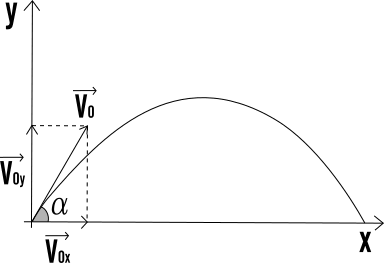
\includegraphics[scale=0.8]{motoParabolico} \end{center}
La cosa fondamentale che vogliamo evincere da questo esperimento è il fatto che ponendoci nelle stesse condizioni: stessa pallina da tennis, stessa posizione all'istante 0 e stessa velocità; il moto sarà sempre identico e la pallina atterrerà sempre nella stessa posizione. Questo ci fa notare come la natura abbia un comportamento deterministico ed è elemento fondamentale del metodo scientifico: se si ottenessero sempre risultati diversi non si potrebbe fare scienza.
\subsubsection{Esperimento quantistico}
Per questo esempio sfruttiamo il già citato esperimento di Zeilinger:
\begin{center} 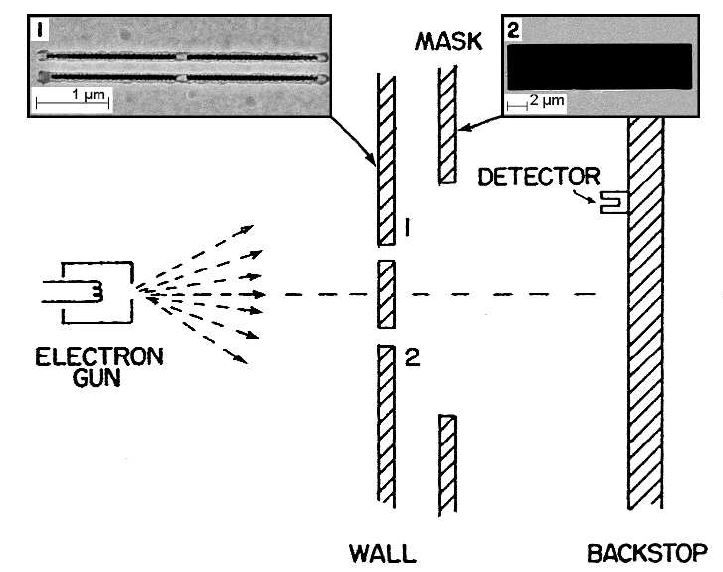
\includegraphics[scale=0.6]{neutronDiffraction} \end{center}
Come si può vedere dall'immagine l'apparato sperimentale è composto da una pistola per neutroni (c'è scritto elettroni, ma il risultato non cambia se si usa una particella oppure l'altra); un muro con due fenditure (che sono dell'ordine di grandezza del diametro della particella), una maschera per evitare al più possibile contaminazioni esterne; un muro finale ove con un detector è possibile trovare la posizione in cui il neutrone è arrivato.
Immaginiamo di esaminare un neutrone per volta; esso è preparato sempre alla stessa maniera e sottoposto sempre allo stesso ambiente; ciò che ci si aspetterebbe, ogni volta misuriamo dove si schianta con il muro finale; compiendo percuò sempre lo stesso identico esperimento quindi ci si aspetterebbe di ottenere sempre lo stesso identico risultato; ma non è così, ogni volta la posizione è diversa.\\
In conclusione non c'è più determinismo, la natura in realtà è casuale e questo è dimostrato empiricamente, quindi non si può più far scienza? Sembrerebbe di no, e sicuramente il percorso del neutrone non è più deterministico e prevedibile con certezza, ma ripetendo l'esperimento un numero molto grande di volte e costruendo un grafico \{numero-neutroni/posizione\} otteniamo un risultato come quello nella figura seguente.
\begin{center} 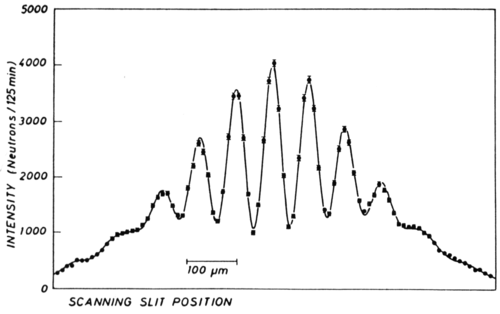
\includegraphics[scale=2.5]{distribuzioneZeilinger} \end{center}
Due sono le osservazioni importanti:
\begin{enumerate}
\item Nel caso in cui si rifacesse tutto da capo otterremmo la stessa identica figura; quindi pur non essendo deterministico un singolo neutrone è possibile fare scienza sulla distribuzione di probabilità di un insieme di essi e quindi descrivere ognuna delle grandezze fisiche di ogni particella come probabilità
\item La figura che si è andata a creare corrisponde esattamente a una figura di interferenza a due fenditure, confermando (come già detto) il dualismo onda-particella
\end{enumerate}
\subsubsection{Limite classico della meccanica quantistica}
A questo punto è necessario chiedersi come mai i modelli matematici applicati a corpi microscopici siano radicalmente diversi da quelli che compongono la fisica classica; in fondo ogni oggetto macroscopico è infine composto da particelle fondamentali che seguono la meccanica quantistica.
Le soluzioni a cui si può arrivare sono molteplici, ma tutte non esaustive, le quali hanno addirittura aperto un dibattito filosofico. Qui però rimaniamo all'interno dell'\textit{interpretazione di Copenaghen}, la più importante. Innanzitutto dato che un corpo macroscopico è formato da un numero enorme di particelle può valere la \textit{legge dei grandi numeri} e quindi ciò che si manifesta non è altro che la "vittoria" dell'evento più probabile. Poi è possibile risalire ad alcune equazione classiche da quelle quantistiche ponendo $\hbar$ $\to$ 0; $\hbar$ è la costante di Planck ridotta, ma non essendo lo scopo dell'elaborato analizzare la matematica dietro la meccanica quantistica l'argomento non verrà approfondito.\\
Il problema che rimane è legato al fenomeno dell'\hyperref[sec:entanglement]{entanglement} che affronteremo fra poco
\subsubsection{Vero stato della materia}
...

\subsection{La sovrapposizione}
Ogni grandezza fisica viene quindi definita e trattata come una distribuzione di probabilità, vediamo cosa un po' più dettagliatemente cosa significa. Come esempio prendiamo lo spin di un elettrone in quanto può assumere solamente due valori: $\frac{1}{2}$ e -$\frac{1}{2}$ al contrario di tante altre che, come ad esempio la posizione, possono assumere infiniti valori continui
\subsubsection{Gli autostati}
Cominciamo a vedere la situazione più semplice: lo spin ha probabilità 1 (o 100\%, è uguale) di essere $\frac{1}{2}$ e probabilità 0 di essere -$\frac{1}{2}$.\\
In questo caso si dice che la grandezza fisica $\textit{spin}$ è in un $\underline{autostato}$ e il valore assunto ($\frac{1}{2}$) è un $\underline{autovalore}$. Quello che accade quindi è che preparando l'esperimento sempre allo stesso l'osservazione dello $\textit{spin}$ produrrà sempre lo stesso risultato.\\
Per estensione qualsiasi grandezza fisica cui la misura di un determinato sistema produce sempre lo stesso risultato (tenendo ovviamente conto degli errori) è un $\underline{autostato}$ indipendentemente da quanti valori la grandezza avrebbe potuto assumere.
\subsubsection{La sovrapposizione}
Quando più valori hanno probabilità non nulla di essere presenti si dice invece che il sistema, per quella grandezza fisica, è in uno stato di $\underline{sovrapposizione}$ (o superposizione dall'inglese $\underline{superposition}$). Ad esempio nel caso la probabilità di ottenere $\frac{1}{2}$ è 0.5 e di -$\frac{1}{2}$ è 0.5 oppure $\frac{1}{2}$: 0.3 e -$\frac{1}{2}$: 0.7 il sistema è in $\underline{sovrapposizione}$. Da ricordare comunque che la somma di tutte le probabilità deve essere sempre 1. Questa però è una semplificazione in quanto in realtà in meccanica quantistica è necessario esprimere le probabilità di ogni valore con numeri complessi rendendo quindi modelli matematici piuttosto complicati, soprattutto in caso di grandezze fisiche continue. A riguardo se ne riparlerà nel capitolo Bit e Qubit nella descrizione di un computer quantistico.\\
Importante ricordare come affermato nell'apposito paragrafico della sotto-sezione precedente che la $\underline{sovrapposizione}$ non esiste in quanto siamo incapaci di preparare in modo preciso l'apparato sperimentale o gli strumenti non sono, ma è un effettivo stato  della materia.\\
Esistono vari modi per produrre uno stato di sovrapposizione con determinate distribuzioni di probabilità in laboratorio, vedremo un esempio nella sezione successiva parlando del principio di Heisenberg
\subsection{La misura}
Nella meccanica quantistica la misura copre un aspetto particolare, piuttosto diverso dalla misura classica.
Infatti in essa è quasi sempre possibile valutare lo stato di un sistema senza perturbarlo negli aspetti interessati; quando non è così la causa sono gli strumenti di misura oppure la perturbazione è determinata e si può risalire matematicamente all'informazione cercata.
In meccanica quantistica invece la misura perturba sempre il sistema e in particolare rompe lo stato di $\underline{sovrapposizione}$ e lo rende un $\underline{autostato}$ con ogni volta un diverso $\underline{autovalore}$ secondo la distribuzione di probabilità.
Questo è molto importante in quanto la trasformazione applicata dalla misura non è prevista dalle varie equazioni (ad esempio quella di Schrodinger) per la trasformazione di un sistema quantistico e non ha una spiegazione logica; diventando quindi il punto di partenza per teorie esotiche come il multimondo (in cui in più universi paralleli si presentano i vari $\underline{autovalori}$
\section{Conseguenze apparentemente controintuitive}
\subsection{Indeterminazione di Heisenberg}
\subsection{Entanglement}
\label{sec:entanglement}
\subsubsection{Il gatto di Schrodinger: vivo o morto?}

\chapter{Bit e Qubit}
Un computer, classico o quantistico che sia, ha lo scopo di gestire e manipolare informazioni; le quali come unità di misura fondamentale hanno il \underline{BIT} (dall'inglese Binary digIT).\\
Nei computer quantistici viene però usata una variante denominata \underline{QUBIT} (QUantum BIT), la quale ha comportamenti di tipo quantistico.
\section{Bit}
\subsection{Boh}
Un bit, sumbolo \textit{b}, può assumere solamente 2 valori: \{\textit{0}, \textit{1}\}, ma è sufficiente per svolgere ogni processo e rappresentare ogni tipo di informazione, qualche esempio:
\begin{enumerate}
\item I numeri (in formato binario) si possono ottenere direttamente con una sequenza di bit, e si possono convertire facilmente in decimale per facilitare la comprensione umana:\\
\textsc{0 = 0}; \textsc{1 = 1}; \textsc{10 = 2}; \textsc{1011 = 11}...
\item Le stringhe (parole, frasi ecc...) non sono altro che insieme di caratteri. Questi ultimi sono rappresentati come numeri e quindi come insiemi di bit; le tabelle di conversione più famose e usate sono la \textit{ASCII} e la \textit{UNICODE}; ad esempio in \textit{ASCII}:\\
97 = \textit{a} ; 125 = \textit{\}} ; 32 = [\textit{Space}]\\
\item Anche le immagini non sono altro che insiemi di numeri; esse sono infatti formate da pixel, ognuno dei quali è composto da tre numeri: componente rossa, componente verde e componente blu; sono difatti matrici tridimensionali. Ovviamente più pixel ci sono più l'immagine sarà di alta qualità, ma comunque se ingrandita ad un certo punto si nota come sia composta da piccoli quadrati. Esiste però un modo di evitarlo per alcune immagini definite e ben conosciute (ad esempio i caratteri) ed è quello di descrivere l'immagine tramite una funzione che definisce un numero definito di pixel (in modo che non siano visibili) indipendentemente dallo zoom.
\end{enumerate}
In quanto unità molto piccola si parla molto più spesso dei multipli dei bit, piuttosto che di essi stessi; i quali però seguono regole un po' particolari rispetto alle grandezze fisiche:\\
Il \textit{Byte}, simbolo \textit{B} è composto da 8 bit e quindi può contenere $2^8 = 256$ diverse combinazioni e quindi rappresentare numeri tra 0 e 255.\\
I prefissi utilizzati sono il \textit{k/kilo-}, il \textit{M/mega-}, il \textit{G/giga-} e il \textit{T/tera-}; ma invece di corrispondere (rispetto al precedente) ad un fattore 1000 come accade solitamente (ad esempio un kilogrammo corrisponde a 1000 grammi) corrispondono ad un fattore 1024; per potersi legare alle potenze di due ($2^{10}$=1024); ad esempio:\\
1 kB = 1024 B; \ 1 MB = 1024 kB = $2^{28}$ bit.
\subsection{Hardware}
L'informazione (i bit) è implementata nella realtà in moltissimi modi che si sono evoluti nell'ultimo secolo; tra i più famosi:
\begin{enumerate}
\item I floppy disk furono tra le più famose unità di memoria negli anni 70 e 80 seppur oggi sono praticamente scomparsi e quasi dimenticati. Erano formati da un disco di materiale ferromagnetico diviso in zone ognuna delle quali per rappresentare i due stati \textit{0} o \textit{1} veniva magnetizzata con il polo nord verso l'alto oppure verso il basso; vantaggio principale era il fatto che poteva essere letto e riscritto un numero teoricamente infinito di volte; però poteva essere facilmente rovinato da campi magnetici ambientali non prevedibili; per di più non permettevano di accedere ad una determinata informazione in modo istantaneo, ma andava ricercata partendo dall'inizio (come accadeva anche per le vecchie videocassette). La capacità media si aggirava intorno ai pochi megabyte.
\item I CD i DVD e i blu-ray sono usati ancora oggi pur molto meno di una decina di anni fa e sono composti da un disco ottico. Cioè per rappresentare 0 o 1 ogni zona può essere bruciata o meno in modo che rifletta oppure no. Le differenze tra loro risiedono soprattutto nella capacità: i CD sono circa 700 MB; i DVD 4 GB e i blu-ray 25GB. Gli hard disk usati nei computer oggi non sono altro che tanti dischi.
\item La memoria flash è la più utilizzata attualmente; ne fanno uso le chiavette USB, le SD card e gli SSD. Ogni bit è composto da un insieme di 5 transistor e questa è la tecnologia migliore; consuma meno, è più affidabile e può avere maggiore capacità. Il problema principale è che la memoria flash non è persistente, ma nel giro di 10-20 anni può perdere informazione. Costa anche un po' di più ma data la \textit{Legge di Moore} il costo tende a scendere. La Legge di Moore è una legge empirica che afferma che circa ogni due anni è possibile produrre transistor di dimensioni dimezzate; il che permette capacità maggiori a costo inferiore. La capacità della memoria flash è infatti molto variabile ed esistono dispositivi di ogni taglia, ma gli SSD più capienti in genere sono dell'ordine del TB.
\item Una menzione va fatta anche alla RAM; essa somiglia alla memoria flash, ma è molto più veloce; è possibile accedere a qualsiasi informazione nell'ordine dei nanosecondi, nei computer attuali ne sono presenti diversi GB. La nota negativa (a parte il costo) è il fatto che la memoria non è persistente e quindi quando cessa l'alimentazione ogni dato viene perso. Il suo uso è quindi quello di permettere di lavorare in tempo reale su informazioni che poi verranno copiate (=salvate) su altra tipo di memoria.
\end{enumerate}
\section{Qubit}

\chapter{Porte logiche}
Le porte logiche sono particolari meccanismi che applicano trasformazioni a bit o qubit (o coppie di essi) e sono quindi la base di tutte le operazioni complesse svolte dalle macchine di Turing, classiche o quantistiche che siano.
\section{Classiche (1 bit)}
\subsection{NOT}
\begin{center}
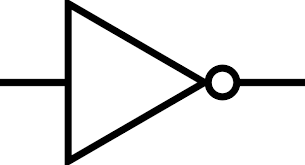
\includegraphics[scale=0.7]{notGate}
\end{center}
La porta logica \textit{NOT} ha in ingresso un segnale e manda in uscita il suo opposto.\\
Mappa quindi:
$0\rightarrow1$ e $1\rightarrow0$.
\section{Classiche (2 bit)}
\subsection{AND}
\begin{center}
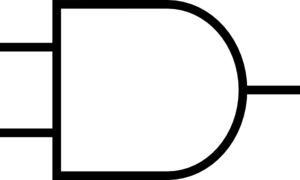
\includegraphics[scale=12]{andGate}
\end{center}
La porta logica \textit{AND} ha in ingresso due segnali e manda in uscita un segnale positivo se e solo se entrambi sono positivi.\\
Mappa quindi:\\
$\{1,1\}\rightarrow1$, $\{1,0\}\rightarrow0$, $\{0,1\}\rightarrow0,$ $\{0,0\}\rightarrow0$
\subsection{OR}
\begin{center}
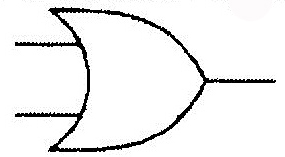
\includegraphics[scale=3]{orGate}
\end{center}
La porta logica \textit{OR} ha in ingresso due segnali e manda in uscita un segnale positivo se almeno uno è positivo.\\
Mappa quindi:\\
$\{1,1\}\rightarrow1$, $\{1,0\}\rightarrow1$, $\{0,1\}\rightarrow1,$ $\{0,0\}\rightarrow0$
\subsection{XOR}
\begin{center}
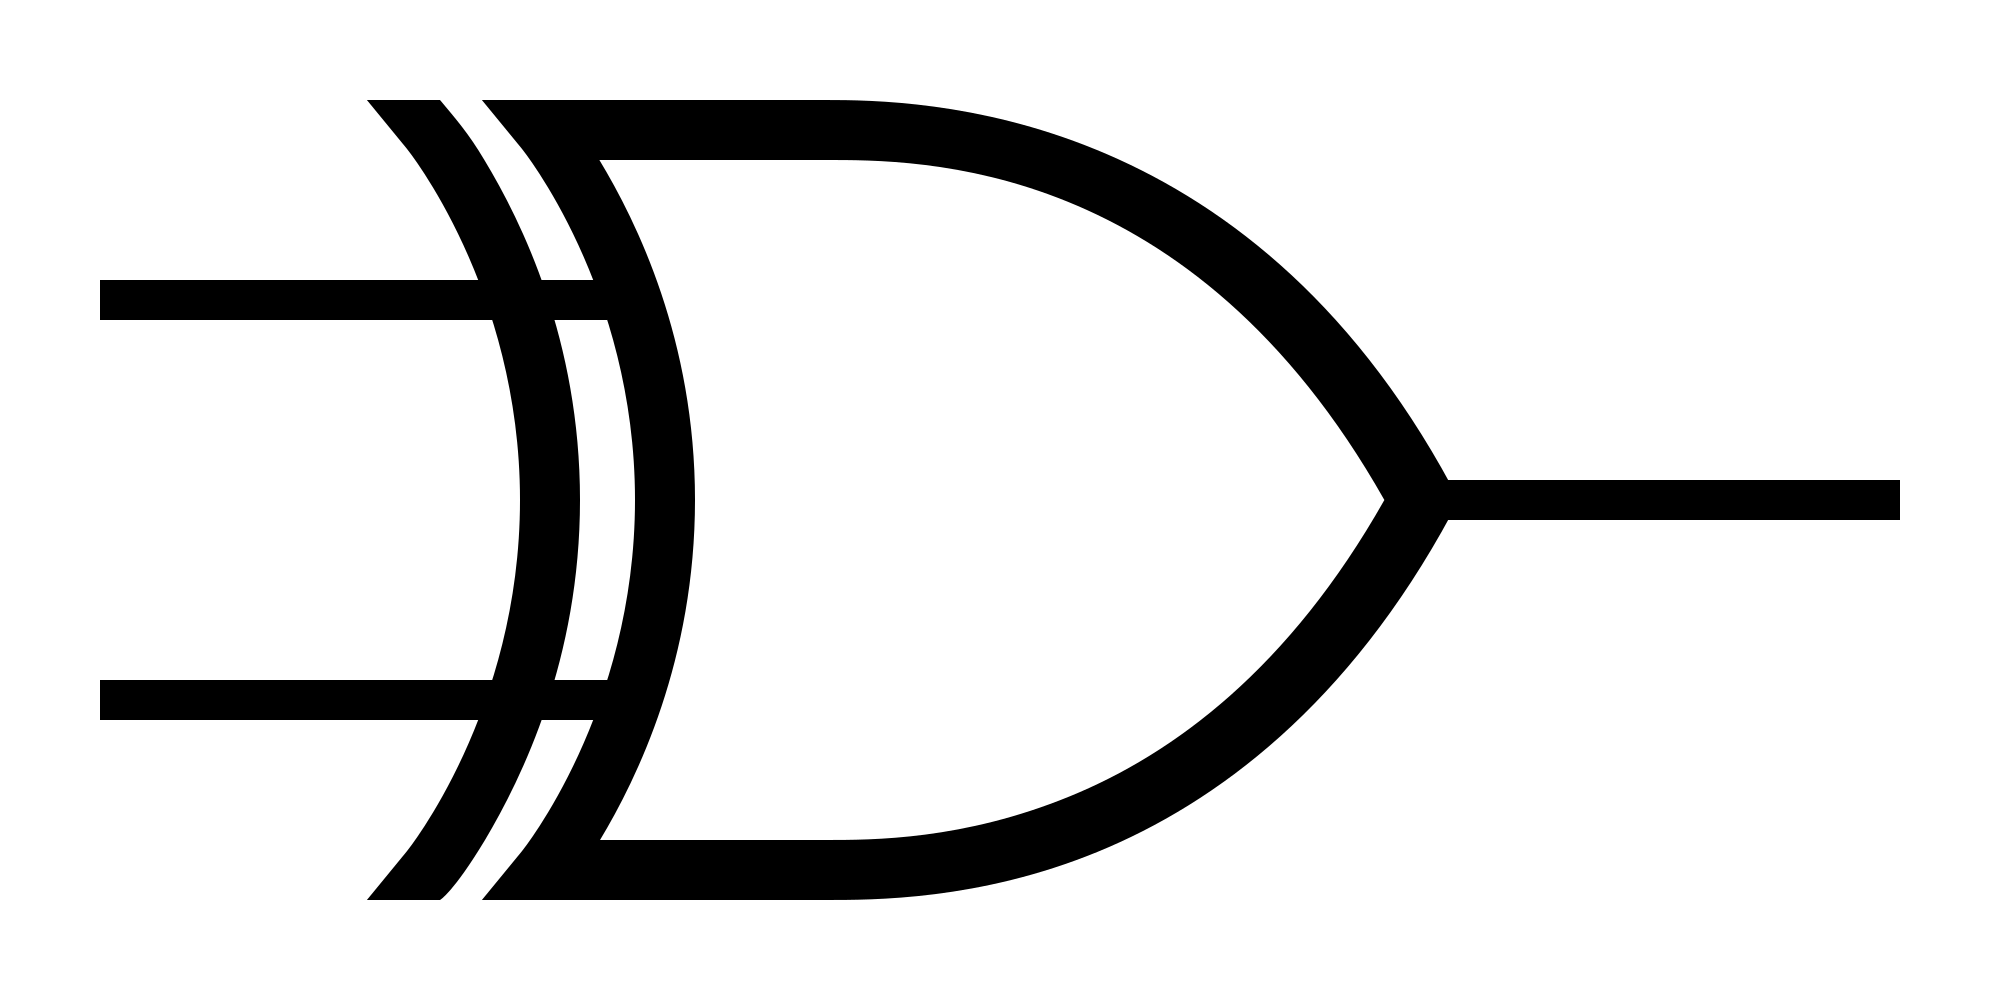
\includegraphics[scale=0.13]{xorGate}
\end{center}
La porta logica \textit{XOR} ha in ingresso due segnali e manda in uscita un segnale positivo se e solo se solo uno è positivo.\\
Mappa quindi:\\
$\{1,1\}\rightarrow0$, $\{1,0\}\rightarrow1$, $\{0,1\}\rightarrow1,$ $\{0,0\}\rightarrow0$
\subsection{Altre}
Esistono poi altre porte logiche, come la NAND o la NOR; ma non sono fondamentali in quanto ottenibili da una combinazione di quelle mostrate (ad esempio NAND = AND + NOT).\\
Porte logiche con più di due segnali di ingresso non vengono usate in quanto per computare più informazioni è sufficiente concatenare.
\section{Quantistiche (1 qubit)}
\subsection{Measurment}
Si tratta della misura di un qubit; non esattamente una porta logica, ma nel capitolo \textit{Cenni di meccanica quantistica} abbiamo visto che applica una trasformazione; misurando infatti il qubit collassa in autostato $\ket{0}$ oppure in $\ket{1}$ con una distribuzione di probabilità dipendente dallo stato del qubit. Per di più il valore viene salvato in un bit classico. Mappa quindi:\\
$\alpha\ket{0} + \beta\ket{1} \rightarrow \ket{0}$ con una probabilità di $|\alpha|^2$ oppure $\alpha\ket{0} + \beta\ket{1} \rightarrow \ket{1}$ con una probabilità di $|\beta|^2$
\subsection{X}
\begin{center}

\includegraphics[scale=1.25]{xGate}
\end{center}
La porta logica \textit{X} è conosciuta anche come \textit{bit-flip} in quanto inverte 0 con 1 e viceversa; è molto simile quindi alla porta classica \textit{NOT}. Mappa:\\
$\ket{1} \rightarrow \ket{0}$\\
$\ket{0} \rightarrow \ket{1}$\\
$\alpha\ket{0} + \beta\ket{1} \rightarrow \beta\ket{0} + \alpha\ket{1}$\\
La porta \textit{X} sulla BLOCH SPHERE applica una rotazione di $\pi$ radianti attorno all'asse x come si può vedere nell'immagine sottostante.
\begin{center}
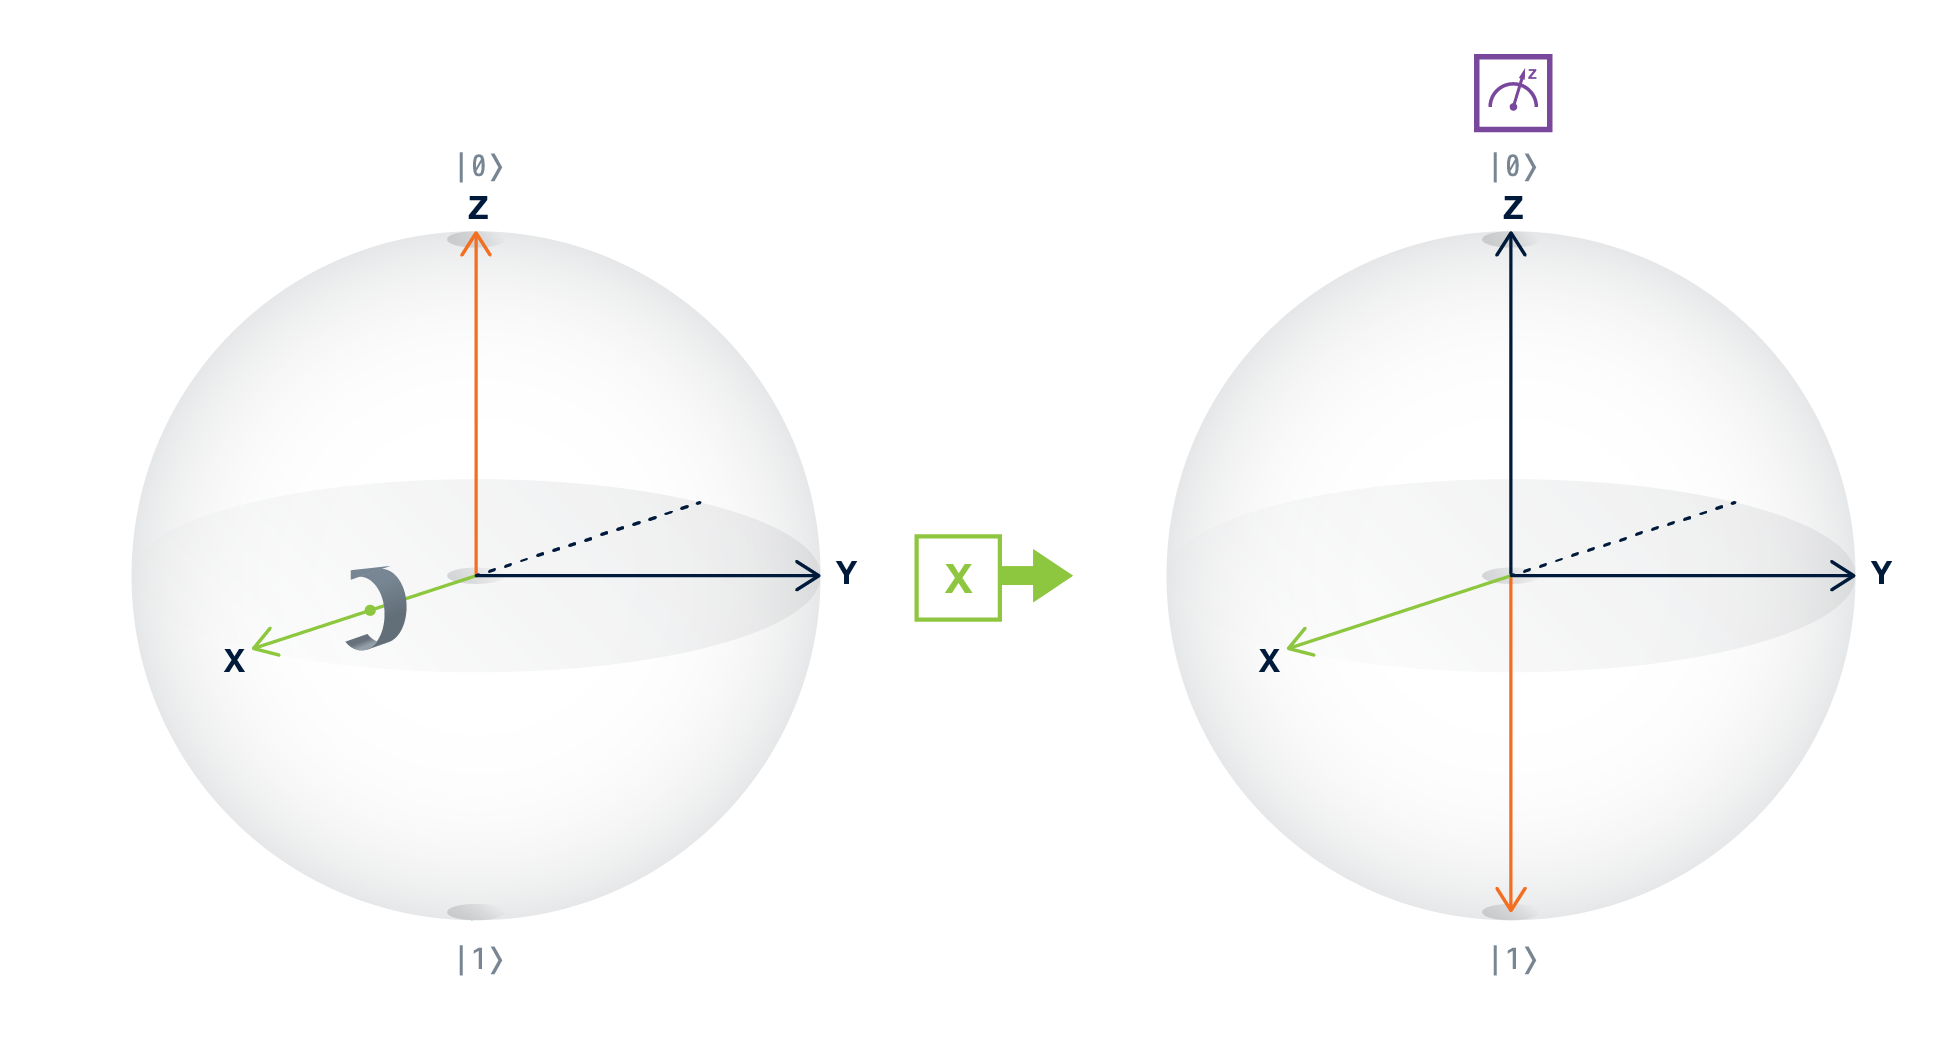
\includegraphics[scale=0.5]{xTrasformation}
\end{center}
\subsection{Hadamard}
\begin{center}

\includegraphics[scale=1]{hGate}
\end{center}
La porta di \textit{Hadamard} (o semplicemente \textit{H}) è forse la più importante delle macchine quantistiche in quanto permette al qubit di passare da un autostato a una superposizione in cui 0 e 1 sono equiprobabili (non sarà ovviamente così se il qubit di partenza non è in un'autostato). Più precisamente si può osservare sulla BLOCH SPHERE che \textit{H} applica una rotazione di $\pi$ intorno agli assi X e Z.\\
Quello che accade agli autostati se applicato \textit{H}:\\
$\ket{0} \rightarrow \frac{1}{\sqrt{2}}(\ket{0} + \ket{1}) = \ket{+}$\\
$\ket{1} \rightarrow -\frac{1}{\sqrt{2}}(\ket{0} + \ket{1}) = \ket{-}$\\
$\ket{+}$ e $\ket{-}$ sono simboli rappresentanti i due vettori di stato che sulla BLOCH SPHERE puntano a +X e a -X. Da notare come $\frac{1}{\sqrt{2}}^2 = \frac{1}{\sqrt{2}}^2 = \frac{1}{2}$ e quindi in entrambi i casi 0 e 1 sono equiprobabili
\begin{center}
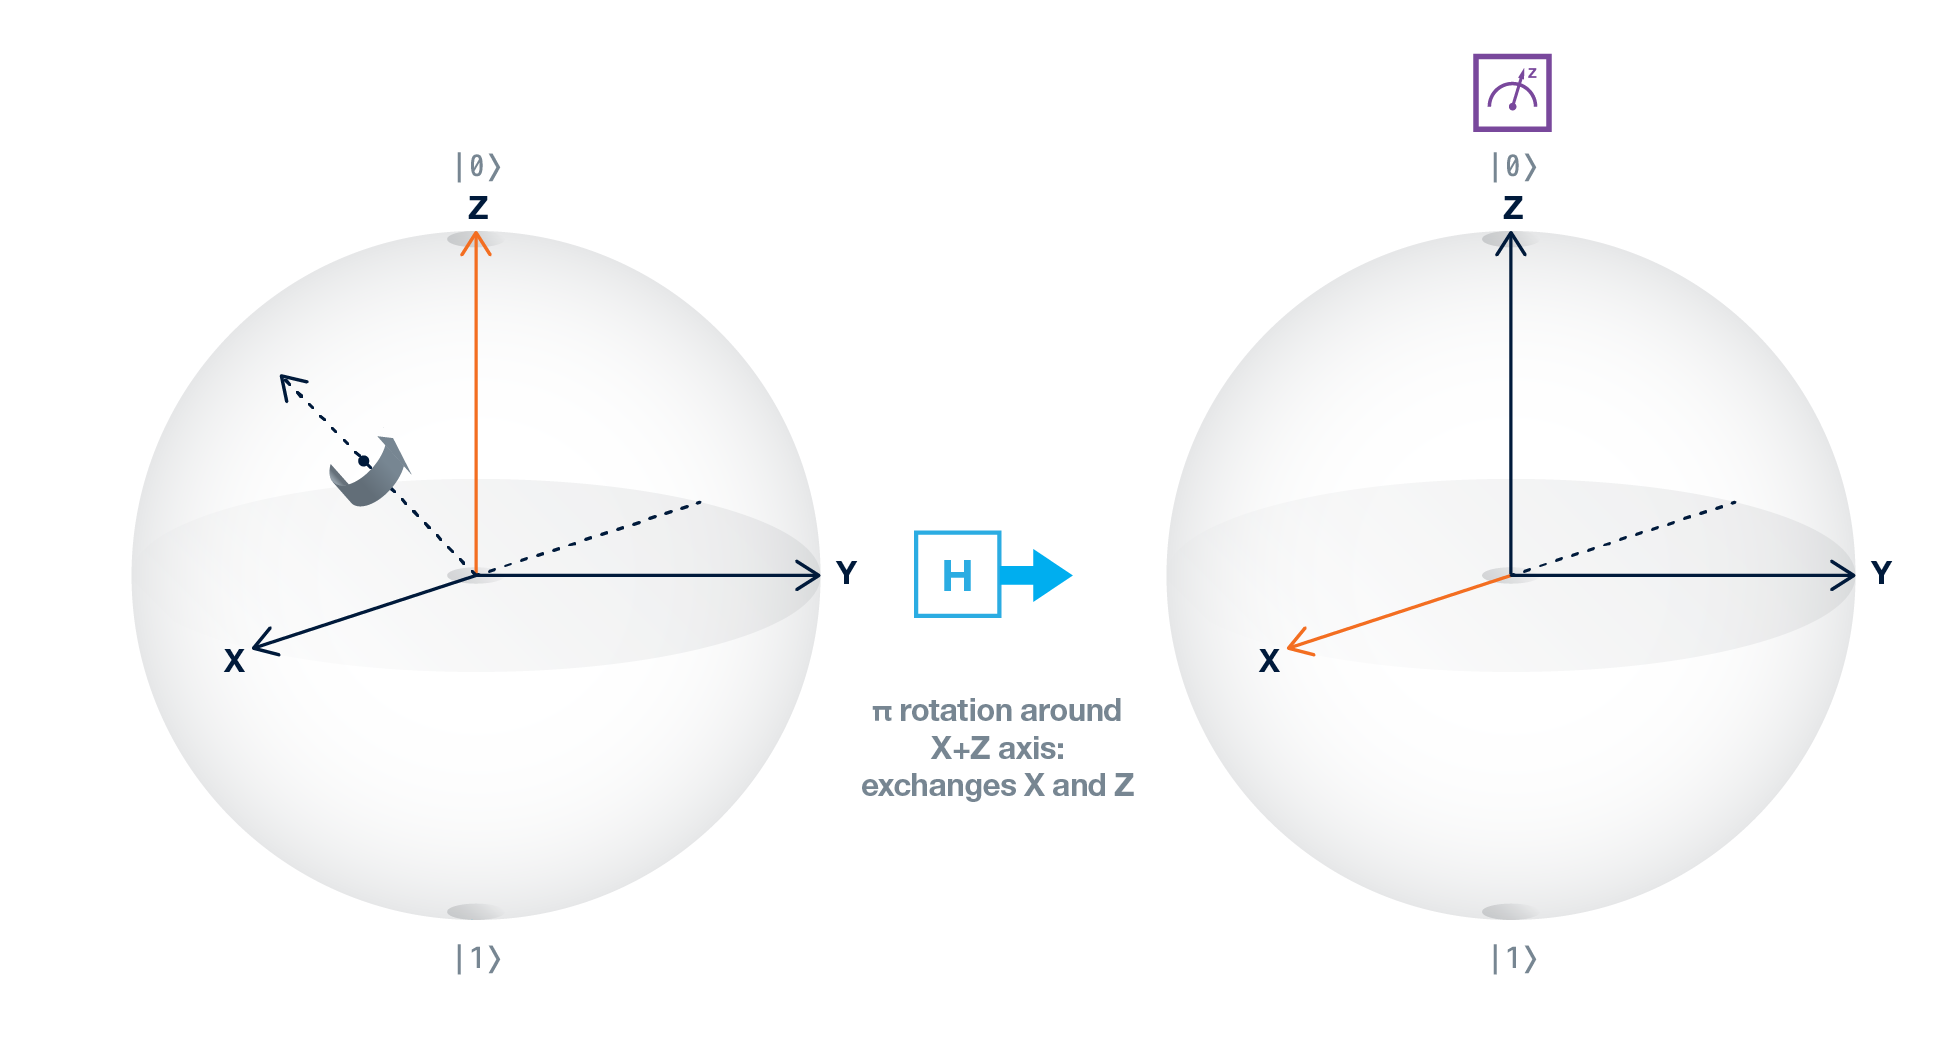
\includegraphics[scale=0.5]{hTrasformation}
\end{center}
\subsection{Z}
\begin{center}

\includegraphics[scale=0.77]{zGate}
\end{center}
La porta \textit{Z} porta ad una rotazione di $\pi$ intorno all'asse Z; gli autostati, essendo allineati, non vengono trasformati come si vede nell'immagine qui sotto.
\begin{center}
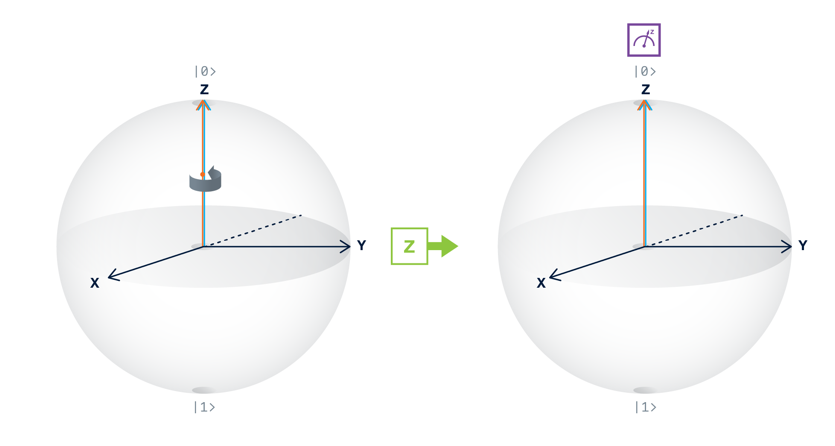
\includegraphics[scale=1.1]{zTrasformation}
\end{center}
Subiscono un effetto invece tutti gli altri vettori di stato, in particolare $\ket{+} \rightarrow \ket{-}$ e viceversa.
\begin{center}
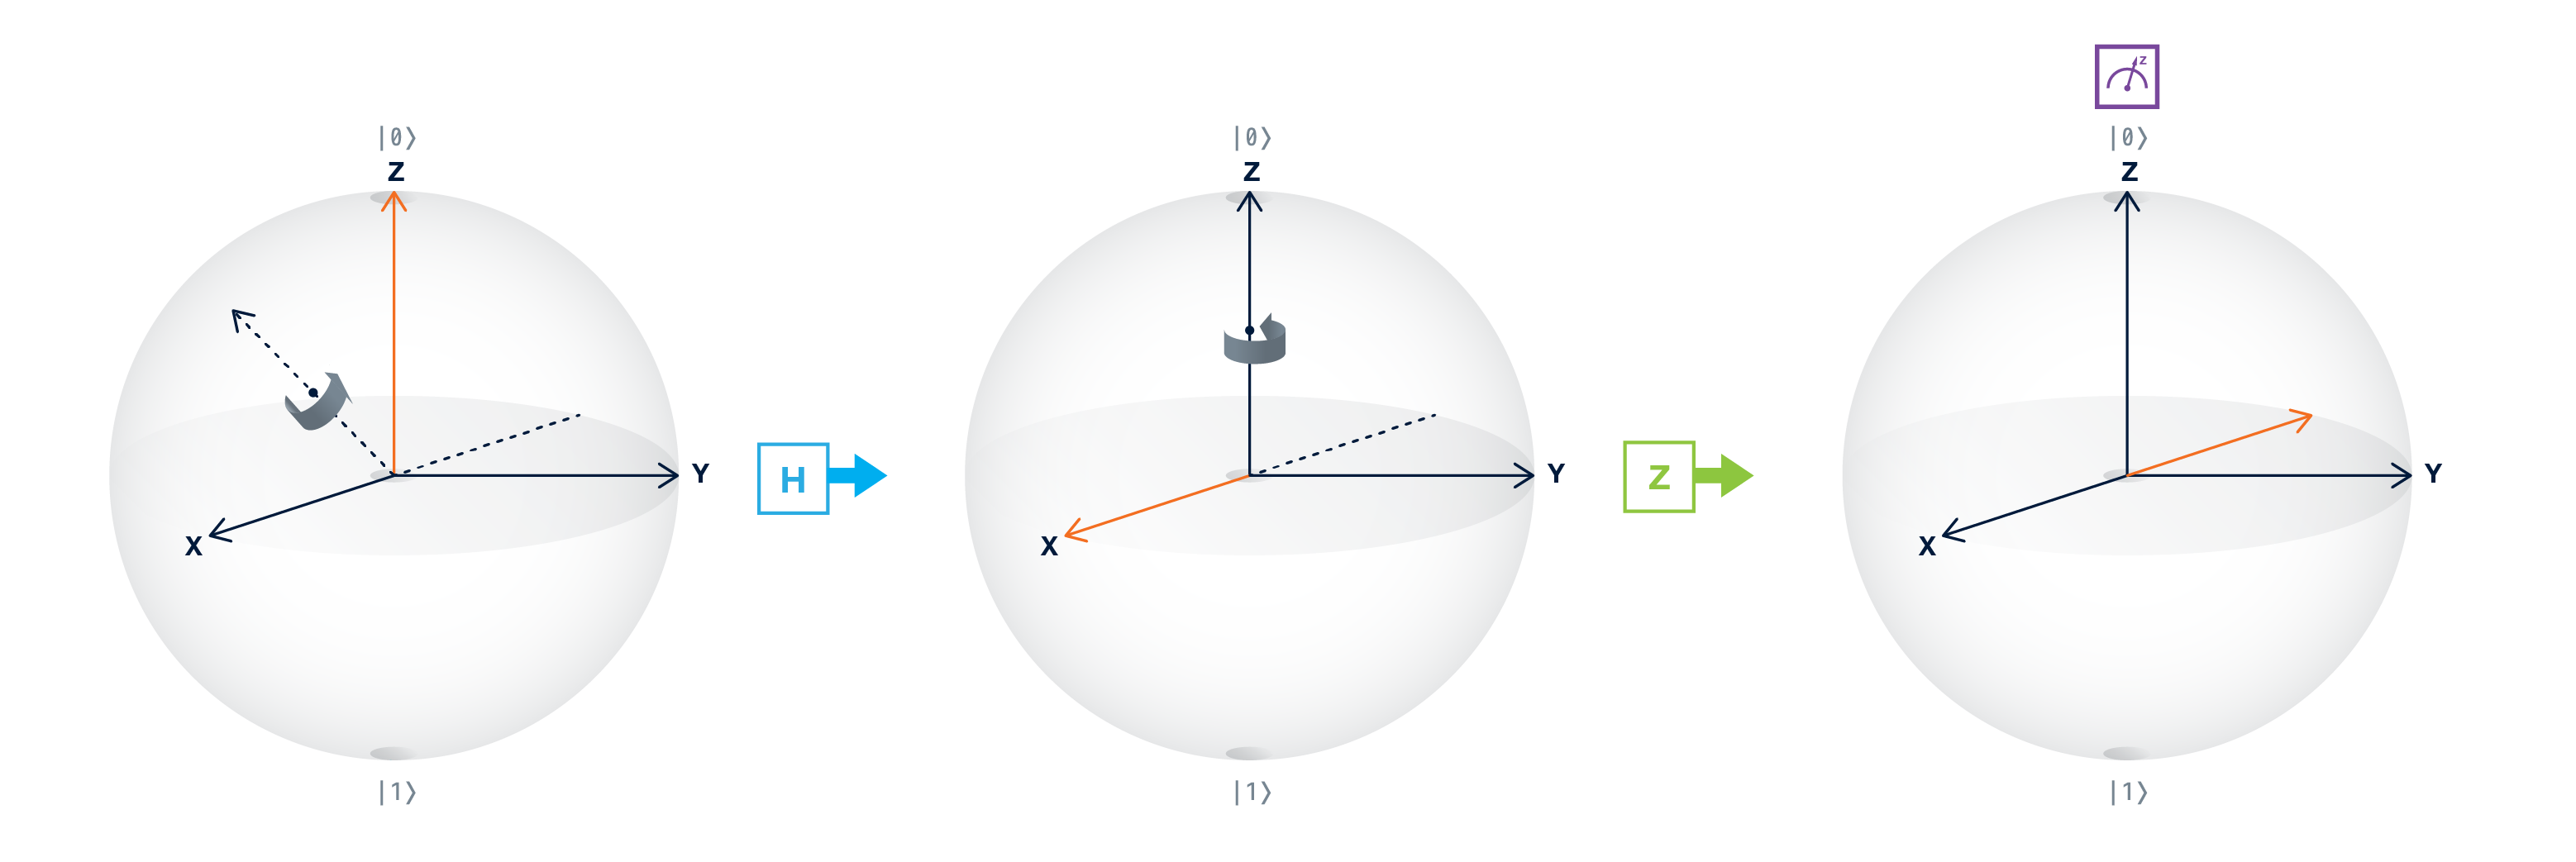
\includegraphics[scale=0.35]{hzTrasformation}
\end{center}
\subsection{S,T}
\begin{center}

\includegraphics[scale=0.77]{sGate}

\includegraphics[scale=0.77]{tGate}
\end{center}
I gate \textit{S} e \textit{T} sono molto simili a \textit{Z} solamente che applicano una rotazione rispettivamente di $\frac{\pi}{2}$ e $\frac{\pi}{4}$ intorno all'asse Z. Nell'immagine i vari esempi a partire da da $\ket{+}$
\begin{center}
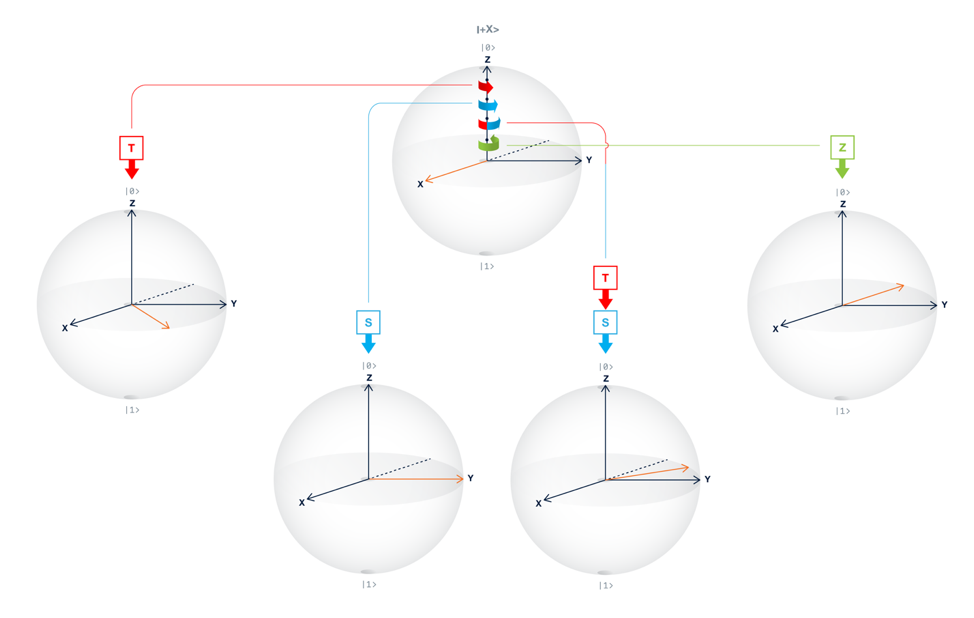
\includegraphics[scale=1.1]{stTrasformation}
\end{center}

\section{Quantistiche (2 qubit)}
Qui tratteremo di due qubit contemporaneamente; gli autostati saranno quindi 4 diversi: $\ket{00}$, $\ket{01}$, $\ket{10}$ e $\ket{11}$. Per convenzione il qubit più significativo (e quindi il primo) si trova nella posizione a destra mentre il secondo a sinistra.\\
Un esempio di sovrapposizione può essere: $\frac{1}{\sqrt{2}}(\ket{00} -\ket{11})$ in cui al 50\% \textbf{entrambi} i qubit varranno 1 e al 50\% \textbf{entrambi} varranno 0. 
\subsection{CNOT}
Le porte di interesse che lavorano su coppie di qubit devono operare della logica condizionale tra i qubit e quindi far dipendere lo stato di uno (chiamato target) da quello dell'altro (chiamato controllo). La porta utilizzata è denominata \textit{Controlled-NOT} o più semplicemente \textit{CNOT}. Essa applica una porta \textit{X} al target se e solo se il controllo assume valore 1, mentre non fa nulla in caso sia 0.\\
Se si abbiano autostati la faccenda è piuttosto semplice: (il qubit di controllo è quello più significativo, mentre il target è quello meno.)
\begin{center}
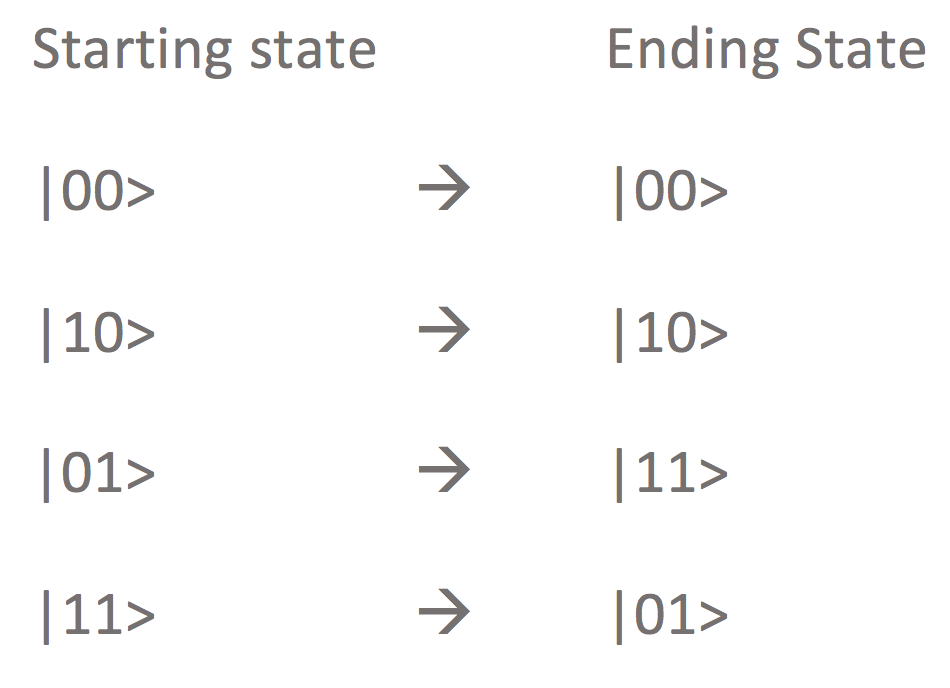
\includegraphics[scale=0.8]{cnotAuto}
\end{center}
Se però il qubit di controllo si trova in uno stato di sovrapposizione tutto diventa più complicato in quanto non si sa a priori se esso valga 0 oppure 1 e quindi nemmeno se il target è stato sottoposto ad \textit{X} oppure no. Chiaramente la misura di anche solo uno dei due fa collassare ad autostato entrambi in quanto conoscere se \textit{X} è stato applicato e che il controllo valga 1 è la stessa cosa.\\
Di particolare importanza è notare come applicare la porta CNOT crei uno stato \textit{entangled} tra i due qubit, peculiaretà che tra bit classici non può in alcun modo accadere.
\chapter{Algoritmi e complessità}
\section{Definizioni e Esposizione dei concetti}
\subsection{Algoritmo}
Per definizione un algoritmo è una sequenza finita di passi base, o operazioni, utili a risolvere un problema, in genere matematico. Essi sono di fondamentale importanza in quanto possono essere la formalizzazione di operazioni svolte da un computer e l'informatica (almeno nella sua parte più scientifica) è la disciplina che li tratta. Storicamente i passi base sono diventati sempre più astratti: se inizialmente trattavano della gestione della memoria byte per byte e di operazioni come porte logiche ad oggi il linguaggio è sempre più matematico e discorsivo non esplicitando quello che avviene a livello hardware. Essendo i computer e la computazione quantistica una tecnologia a livello ancora "embrionale" e di fatto molto più complessa del corrispettivo classico un linguaggio astratto non è ancora sviluppato.
\subsection{Complessità}
La complessità è una proprietà di ogni algoritmo ed indica quanto veloce o lento esso viene eseguito (si parla di complessità temporale) oppure quanta memoria deve occupare (si parla di complessità di memoria).
In genere la memoria è di secondaria importanza in quanto i calcolatori attuali (soprattutto se si prendono in considerazione i supercomputer) ne dispongono di sufficiente per la maggior parte dei problemi, ma la complessità temporale è fondamentale in quanto un particolare problema è necessario che sia risolto oggi e non tra qualche anno o addirittura nemmeno domani.\\
Essa viene espressa da una funzione \textit{T(N)} tempo su dimensione dei dati in input. Dovendo un algoritmo risolvere non solo un'istanza di un problema, ma tutti i casi possibili chiaramente il tempo impiegato dipende anche dai dati di partenza; in particolar modo dalla loro quantità e dimensione (cioè quanta memoria occupano). Essendo ogni calcolatore diverso e diventando più potenti con l'avanzare del tempo \textit{T(N)} non viene espresso in secondi dato che sarebbe diverso per ogni hardware, ma in numero di passi base che dipende solo dall'algoritmo in sè. Anche questo metodo è però troppo specifico in quanto esprimere \textit{T(N)} può essere molto difficile oppure pieno di dati poco importanti; viene quindi usata la notazione \textit{O-grande} cioè una funzione \textit{O(f(N))} che esprime l'andamento della complessità, più precisamente:
$T(N) := O(f(N)) \iff \exists \ C\times f(N) > T(N)\ \forall \ N \geq n0 \ | \ C,n0 \in \ \mathbb{R} $\\
Cioè un algoritmo si può dire \textit{O(f(N))} se e solo se f(n) moltiplicato per una certa costante è sempre maggiore di \textit{T(N)} da un certo punto in poi. Questa notazione è ottima in quanto dove non funziona (cioè per N molto piccoli) il tempo impiegato è talmente poco che non ci si può accorgere dell'errore e dove funziona (per N grandi) esprime con semplicità e ottima approssimazione il tempo impiegato (eliminando fattori di poca importanza).\\
Tutti i problemi del mondo vengono classificati in relazione alla complessità migliore ottenibile dagli algoritmi risolventi; una prima distinzione viene fatta tra i problemi non calcolabili e quelli calcolabili, cioè quelli per cui non può e può esistere un algoritmo risolvente. Poi ognuno dei calcolabili appartiene all'insieme \textbf{NP} (Non Polinomiale) in cui può esistere un algoritmo in grado di risolvere i problemi con una complessità non polinomiale (cioè in \textit{O(f(N))} f(N) non è polinomiale) e un sottoinsieme di essi appartiene anche a \textbf{P} (Polinomiale) ove può esistere un algoritmo in grado di risolverli in tempo polinomiale. Da porre attenzione però al fatto che polinomiale e non polinomiale in questo caso non hanno il vero significato matematico in quanto all'insieme dei polinomiali appartengono anche alcune funzioni come le logaritmiche; per NP si intende più che altro funzioni che crescono più velocemente delle polinomiali.\\
All'interno di P si distinguono poi numerosissime classi a seconda delle  varie f(N), di seguito un elenco delle più famose (in ordine dalla più veloce):\\
\textit{O(1)}, \textit{O(logN)}, \textit{O($\sqrt{N}$)}, \textit{O(N)}, \textit{O(NlogN)}, \textit{O($N^2$)}, \textit{O($N^k$)}...
\section{Esempi classici}
Alcuni esempi di algoritmi classici. La somma con le porte logiche, la ricerca lineare e la ricerca binaria.
\subsection{Somma}
Sommare due numeri è relativamente semplice per il cervello umano, ma non immediato per una macchina; ricordiamo infatti che le uniche operazioni che può fare in modo diretto tra bit sono date dalle porte logiche e quindi bisogna trovare un modo di combinarle per fare in modo che a partire da due bit si ottenga la somma.\\
Per capire meglio partiamo dall'esempio di voler sommare 6 e 7, a mente il risultato è immediato, ma basiamoci sulla struttura delle somme in colonna:
\begin{lstlisting}[language=python]
   6
+  7
----
= 13
\end{lstlisting}
Il ragionamento è che 6+7 vale 3 con il resto di 1 che va portato alla colonna successiva in cui non c'è nulla e quindi alla fine 13.\\
I numeri sono però in formato binario nei computer, ma non è un problema in quanto la regola vale comunque, è anzi più semplice in quanto ci sono solo due possibili cifre; 6 è 110, mentre 7 111:
\begin{lstlisting}[language=python]
   110
+  111
------
= 1101
\end{lstlisting}
Il ragionamento è che 1+0 sia 1 senza resto, poi 1+1 sia 0 con il resto di 1 e infine 1+1+1 è 1 con il resto di uno che rimane su una colonna vuota; quindi il risultato è 1101, il corrispondente di 13.\\
Partendo da analizzare una sola colonna si ha bisogno di un circuito che dati due bit di partenza dia come risultato 1 se solo uno dei due vale 1 (e quindi una porta \textit{XOR}), 0 altrimenti e come resto 1 solo se entrambi valgono 1 (quindi una porta \textit{AND}). Nell'immagine qui sotto A e B sono gli input mentre S il risultato e C il resto. Il rettangolo con la scritta "Half Adder" è il riassunto del circuito sopra con a sinistra gli input e a destra gli output.
\begin{center}
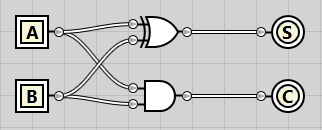
\includegraphics[scale=1.3]{halfSum}\\
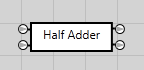
\includegraphics[scale=1]{halfSumIco}
\end{center}
Questo circuito però non basta a sommare una colonna qualsiasi in quanto potrebbe esserci il resto dalla colonna prima, è quindi necessario un circuito piò complicato, chiamato "Full Adder". I quadrati A (primo bit), B (secondo bit) e C (resto precedente) sono gli input, i cerchi S e C gli output.
\begin{center}
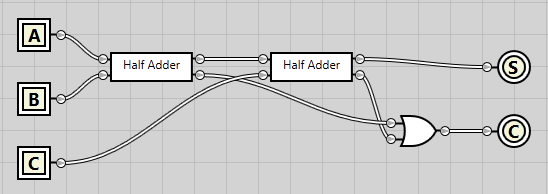
\includegraphics[scale=0.9]{fullAdder}
\end{center}
Ora che è possibile sommare una colonna per sommarne di più basta concatenare i "Full Adder" in modo  che il resto ogni volta faccia parte della colonna successiva; ad oggi i processori sono disegnati per maneggiare fino a 64 bit per volta, ma nell'immagine qui sotto un esempio di 3, in cui si svolge 7+3 (il rosso corrisponde a 1, il bianco a 0):
\begin{center}
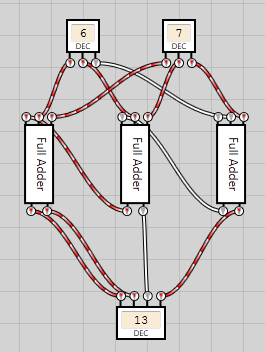
\includegraphics[scale=0.9]{triAdder}
\end{center}
\subsection{Ricerca lineare}
Data una lista casuale di elementi determinare se un preciso elemento denominato X esiste e in che posizione si trova.\\
Questo problema viene risolto da un algoritmo di ricerca molto semplice: controllare ogni elemento partendo dal primo e verificare se esso è uguale ad X; in pseudo-codice:
\begin{lstlisting}[language=python]
posizione = None
contatore = 1
for elemento in lista:
	if elemento = X:
		posizione <- contatore
	contatore = contatore + 1
return posizione
\end{lstlisting}
Dovendo potenzialmente analizzare tutta la lista la complessità di questo algoritmo è \textit{O(N)}
\subsection{Ricerca binaria}
Il problema cui si vuole trovare soluzione è lo stesso dell'esempio precedente, ma la lista, invece che essere casuale, è ordinata. Certamente la ricerca lineare funzionerebbe comunque, ma nello specifico caso è possibile usare una variante più efficiente.\\
Invece di iniziare dal primo elemento si parte da quello centrale e si verifica se si trova prima o dopo dell'elemento cercato (se sono numeri ad esempio si controlla se è maggiore o minore) e si restringono gli estremi della lista di conseguenza; se ad esempio l'elemento si trova primo di quello centrale si può eliminare dalla ricerca la seconda metà della lista. Lo stesso procedimento si applica a ripetizione continuando ad accorciare la lista di interesse. In questo modo è anche possibile trovare la posizione che occuperebbe l'elemento in caso non sia presente oppure gli elementi più simili. Nell'esempio qui sotto viene trovata la posizione dell'elemento minore o uguale ad X:
\begin{lstlisting}[language=python]
inizio = 1
fine = length(lista)
while inizio < fine:
	mezzo = (inizio + fine)/2
	if lista[mezzo] < X:
		fine = mezzo
	else:
		inizio = mezzo
return mezzo
\end{lstlisting}
Si può facilmente dimostrare come con questo algoritmo si venga a creare un albero binario di scelte (difatti ad ogni iterazione si scegle se prendere il sottoinsieme di destra o sinistra) che ha come base gli elementi singoli della lista. Per trovarne uno è necessario percorre tutto un ramo (e quindi l'altezza dell'albero) che è lungo \textit{$\log_22$} volte la base; la complessità è quindi \textit{O(log(N))}
\subsection{Commesso viaggiatore}
Il problema è: Viene data una lista di città e la descrizione delle strade che le collegano; in particolare quali sono e quanto tempo impiegano ad essere percorse. Si vuole trovare il percorso che partendo da una determinata città le attreversi tutte e ritorni impiegando meno tempo possibile.\\
L'unico modo per risolverlo è provare ogni singolo percorso, e, dato che il numero delle combinazioni cresce in modo esponenziale con l'aggiunta di città e strade, il problema rientra nella classe NP. Questo significa che oltre un certo (abbastanza basso) numero di città il tempo che si impiega per calcolare il percorso migliore può essere di anni o anche millenni il che rende (se non nella teoria) nella pratica impossibile risolvere il problema.
\section{Esempi quantistici}
Le macchine quantistiche hanno la possibilità di sfruttare ogni algoritmo classico (ma non conviene in quanto sono molto più costose e difficili da costruire), però non è vero il contrario; esistono algoritmi che possono essere eseguiti solo da computer quantistici.
Questi ultimi in genere risolvono alcuni problemi calcolabili con una complessità minore degli algoritmi classici; in particolare un sottoinsieme dei Non Polinomiali (chiamato EQP) se approcciato con una macchina quantistica rientra nei Polinomiali. (Questo ovviamente non funziona per tutti i problemi, ad esempio il commesso viaggiatore rimane NP).\\
Essendo la maggior parte di questi algoritmi molto complessi sia dal punto di vista informatico che matematico (richiedendo conoscenza approfondita di algebra lineare) gli algoritmi non verranno approfonditi, ma solo esposti.
\subsection{Deutsch-Josza}
Disponiamo di una scatola nera che implementa una funzione \textit{$f: \{0,1\}^n \rightarrow \{0,1\}$} cioè prende in input \textit{n} bit e ha un output di uno solo. Di questa funzione si sa solo che può essere o costante (cioè per tutti gli input restituisce un solo risultato) oppure bilanciata (e quindi per esattamente metà restituisce 1 e per l'altra metà 0). Viene richiesto quindi di determinare se \textit{f} è costante o bilanciata.
Questo è il problema che l'algoritmo di Deutsch-Josza deve risolvere.
\subsubsection{Approccio classico}
Innanzitutto si può notare che esso è risolvibile anche in modo classico: si possono provare in ordine varie combinazioni degli \textit{n} bit e verificare come si comporta \textit{f}. Nel caso ottimo bastano due test, se il risultato è diverso sicuramente la funzione non può essere costante e quindi è bilanciata; nel caso pessimo però è necessario provare almeno la metà più uno in quanto finchè otteniamo risultati identici non possiamo essere sicuri che \textit{f} sia costante finchè essi non sono più della metà. La complessità di un approccio classico è infatti \textit{O($2^n$)} in quanto, essendo $2^n$ le possibili combinazioni, ne vanno testate in media $2^{n-1} + 1$.
\subsubsection{Approccio quantistico}
Nel caso in cui la scatola nera sia una macchina quantistica e quindi non rompa la superposizione dell'input è possibile applicare l'algoritmo (quantistico) di Deutsch-Josza. Il concetto è che invece di dare in input una combinazione precisa, ogni singolo qubit è in sovrapposizione con egual probabilità di essere 0 o 1. Si ottiene quindi una correlazione tra input e output la quale ha probabilità di avere valore 0 nulla solo se \textit{f(x)} è bilanciato e valore 1 se \textit{f(x)} è costante (per interferenza distruttiva e costruttiva).
Per più informazioni a riguardo:\\
$\href{https://bit.ly/2MwuZRI}{bit.ly/2MwuZRI}$\\
La complessità di questo algoritmo è \textit{O(N)} in quanto richiede solo di preparare una combinazione, il che è un'accelerazione esponenziale rispetto all'algoritmo classico.
\subsection{Grover}
Per l'algoritmo di Grover il problema è la ricerca in una lista casuale (come la ricerca lineare) con un approccio quantistico.\\
Nell'algoritmo viene costruita una sovrapposizione di qubit in modo tale che ogni indice sia equiprobabile, vengono poi applicate delle trasformazioni al sistema in modo tale che la probabilità dell'indice corretto aumenti; questo viene ripetuto un numero tale di volte da massimizzare la probabilità che il sistema collassi all'indice corretto, si può dimostrare che il numero è dell'ordine di $\sqrt{N}$.
La probabilità di ottenerlo però non arriva mai a 1 e quindi si può ottenere un risultato sbagliato; per questo l'algoritmo non è deterministico, ma dato che essa non dipende da N ripetere l'esecuzione dell'algoritmo solo poche volte rende la probabilità di errore molto prossima allo  0. La complessità dell'algoritmo è quindi \textit{O($\sqrt{N}$)}.
Per approfondimenti:\\
$\href{https://bit.ly/1ubOwWj}{bit.ly/1ubOwWj}$
\subsection{Shor}
Il problema che viene affrontato dall'algoritmo di Shor a parole è relativamente semplice: Fattorizzare un numero. Vediamo innanzitutto come risolverlo da un punto di vista classico.
\subsubsection{Approccio classico}
Non esistendo alcuno stratagemma veloce per determinare quali primi dividono un numero qualsiasi è necessario provare tutti quelli minori del numero da dividere. Sfortunatamente però non esiste nemmeno un modo istantaneo per discernere un numero primo da un non primo e nemmeno uno che ci permette di capire quale sia il numero primo successivo a uno dato; quindi non solo bisogna tentare tutti i primi minori del numero, ma bensì tutti (o quasi) i numeri minori; se ad esempio volessimo scomporre 308 il procedimento sarebbe il seguente:
Si tenta di dividere per 2 308, è possibile quindi 2 è un fattore, otteniamo 154. Si riprova con 2 ed è dividibile, otteniamo 77. Esso non è divisibile per 2, nè per 3, nè per 5, ma invece per 7 sì (si possono saltare i fattori pari) otteniamo 11. Esso non è divisibile per 7, nemmeno per 9 ma per 11; otteniamo 1. Essendo 11 maggiore di 1 possiamo fermarci.\\
308 viene quindi scomposto in $2^2 \times 7 \times 11$. Si può notare come potenzialmente ci si può spingere fino a $\sqrt{M}$ (dove M è il numero) e l'insieme dei numeri compresi tra 2 e $\sqrt{M}$ cresce in modo esponenziale rispetto al numero di cifre (chiamato N) di M, perciò aggiungere una cifra al numero da scomporre rende l'algoritmo esponenzialmente più lento. La complessità si può quindi denotare approssimativamente con \textit{O($2^N$)}.
\subsubsection{Approccio quantistico}
La chiave dell'algoritmo quantistico di Shor sta nel processo di ricerca del periodo di una funzione svolto dalla \textit{trasformata di Fourier quantistica} (\textbf{QFT}). Per capire come essa funzioni riporto l'analogia del professor Scott Aarson tradotta in italiano:
\begin{displayquote}
Immaginiamo che io abbia degli orari molto strani; in particolare la mia giornata dura più di 24 ore. Se ti dicessi che oggi mi sono svegliato alle 5 del pomeriggio sapresti dirmi quanto di preciso dura: 25, 26, 27.4...? Certo che no, infatti in ogni caso la mia sveglia cambierebbe ogni giorno e prima o poi nella maggior parte dei casi capiterà che arrivi alle 5 del pomeriggio.\\
Ora immaginiamo che il muro della mia camera sia pieno di orologi analogici, ma tutti diversi: in ognuno di essi la lancetta delle ore per compiere un giro intero ci impiega un tempo diverso e per di più esiste un orologio per ogni periodo cui si possa pensare. Poi sotto ognuno è presente un poster cui è attaccata una puntina. Ti posso assicurare che la prima volta che ho dormito nell'appartamento ho posizionato le puntine al centro di ogni poster, poi però ogni giorno subito dopo essermi svegliato spostavo le puntine di un centimetro nella direzione indicata dalla lancetta.\\
Ora, esaminando le puntine, si può affermare con sicurezza la durata della mia giornata? Assicuro che sì, è possibile. Per esempio se la mia giornata fossse di 26 ore si può dedurre che il moto della puntina sotto l'orologio delle 24 ore sia periodico; ogni giorno la lancetta punta in posizioni diverse e prima o poi ritornerà nella posizione iniziale.\\
Cosa accade però alla puntina sotto l'orologio delle 26 ore? Essendo in sincrono con la mia giornata ogni volta che mi sveglio la lancetta punta sempre la stessa ora, e quindi la stessa direzione, perciò la puntina si muoverà sempre nella stessa direzione. L'importante è che questo accade solo per l'orologio delle 26 ore.
\begin{center}
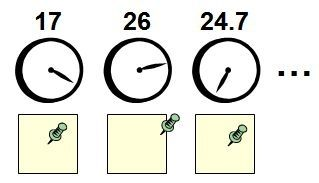
\includegraphics[scale=1]{ShorClocks}
\end{center}
Infine quindi per determinare la durata della mia giornata basta solo cercare l'orologio la cui puntina è più lontana dal punto iniziale.
\end{displayquote}
Questo è quello che accade nel QFT: una serie di qubit in sovrapposizione rappresentano contemporaneamente tutti i possibili periodi, poi per interferenza costruttiva quello corretto diviene sempre più probabile a discapito degli altri, così che quando il sistema collassa molto probabilmente sarà sul periodo corretto.\\
Successivamente ci si può avvalere della matematica classica difatti per fattorizzare un numero \textit{N} basterà scegliere un numero casuale minore di N chiamato \textit{a} e cercare la periodicità di $a^x mod N$ (Dove \textit{mod} rappresenta il resto della divisione. A questo punto è dimostrabile come il Massimo Comun Divisore di $a^\frac{periodo}{2}$-1 e N è un fattore di N e quindi la soluzione.\\
Questo non funziona per tutti gli \textit{a}, ma è molto più probabile un esito positivo piuttosto che negativo; quindi è sufficiente provarne pochi.
Calcolare la complessità non è semplice, in quanto dipende da come l'algoritmo viene implementato, ma dovrebbe essere intorno a \textit{O($N^3$)} il che è un'accelerazione esponenziale rispetto all'algoritmo classico.
Per approfondire:\\
\href{https://bit.ly/2tfo86l}{bit.ly/2tfo86l}
\chapter{Quantum supremacy e applicazione di computer quantistici}
Si parla di Quantum Supremacy (Supremazia quantistica) quando un computer quantistico riesce a risolvere un problema meglio (e in meno tempo) del miglior super-computer classico. Questo periodo (circa la metà del 2018) è di fondamentale importanza in quanto per la prima volta si sta raggiungendo questo obiettivo.
\section{Attualmente}
\subsection{Essere un computer quantistico}
Sembra assurdo, ma ad oggi è l'unica cosa che i computer quantistici riescono a fare meglio di quelli classici; e non è banale.\\
Infatti è possibile con un computer classico simulare in modo perfetto un computer quantistico, ma ovviamente diventa sempre più difficile per ogni qubit che si vuole aggiungere; ad oggi IBM è riuscita a simulare 56 qubits, numero che è quindi diventato spartiacque per la supremazia quantistica: riuscire a costruire una macchina quantistica generica (senza quindi limitazioni o specializzazioni) di almeno 57 qubits vale al raggiungimento della supremazia quantistica.\\
Importante notare come i computer classici non possono evolversi nella simulazione di computer quantistici più velocemente di quanto si evolvono i computer quantistici stessi in quanto l'aggiunta di ogni qubit simulato richiede esponenzialmente più risorse e in particolare se si vuole simulare anche solo 260 qubits sarebbero necessari più bit di quanti atomi sono presenti nell'universo.
\subsection{Sampling problem}
Data una determinata distribuzione di probabilità si vuole avere una funzione che genera valori secondo la determinata distribuzione.\\
Per un computer classico è in realtà un problema piuttosto difficile soprattutto se i possibili valori tra cui scegliere sono molti.\\
Al contrario per un computer quantistico è particolarmente semplice in quanto il problema fa intrinsecamente parte del suo funzionamento; infatti costruendo un sistema di, ad esempio 50 qubit, essi possono rappresentare $2^{50}$ (un numero a 15 cifre) valori contemporaneamente e la probabilità con cui ogni numero si presenta è possibile ottenerla modificando la superposizione dei 50 qubit. In questo modo è quindi possibile costruire una distribuzione di probabilità tra i $2^{50}$ valori e la funzione per ottenerli non è altro che la misura del sistema, in quanto farà collassare i qubit secondo la distribuzione di propabilità costruita.\\
La problematicità sta nel fatto che in realtà questa proprietà è quasi inutile in quanto sono pochissimi i casi di applicazione e dove anche esistono (ad esempio nel campo dell'intelligenza artificiale) il problema ha delle piccole varianti che rendono il tutto più complesso.
\section{In futuro}
\subsection{Crittografia}
La crittografia è il processo di cifrare dei dati, e quindi nasconderli, secondo un criterio (in genere matematico) preciso in modo che la cifratura di dati identici deve portare a risultati identici, e spesso è anche necessario che sia possibile tornare indietro semplicemente.\\
Al giorno d'oggi esistono diversi algoritmi di crittografia; quelli più famosi sono di tre tipi:
\begin{enumerate}
\item Unidirezionali, cioè non è mai necessario che dai dati cifrati si ritorni ai dati in chiaro.\\
Un esempio d'uso riguarda le password: ogni servizio digitale richiede che gli utenti si autentichino utilizzando una password, essa non viene però salvata in chiaro (in quanto è possibile che qualcuno si infiltri e legga), ma cifrata; l'autenticazione avviene confrontando se cifrando quello che l'utente inserisce si ottiene lo stesso risultato della versione salvata.
\item A chiave simmetrica, cioè la cifratura avviene secondo un criterio che quando semplicemente invertito permette di decifrare.\\
Un esempio famoso è il cifrario di Cesare in cui ogni carattere del messaggio da cifrare viene spostato di 13 posti nell'alfabeto verso destra. Ovviamente è sufficiente andare verso sinistra per riottenere il messaggio in chiaro.\\
Questo genere di cifratura non viene praticamente mai usato in quanto poco sicuro
\item A chiave asimmetrica, cioè esiste una chiave in grado di cifrare i dati e una in grado di decifrarli, ma esse non sono correlate in modo semplice ed è quindi impossibile risalire dalla chiave di cifratura (chiamata anche pubblica) a quella di decifratura (o privata).\\
Questi algoritmi sono in genere utilizzati nelle comunicazioni in quanto ad esempio se A e B vogliono comunicare possono per prima cosa scambiarsi le chiavi pubbliche, poi quando A vuole scrivere a B utilizza per cifrare la chiave di B, poi B può decifrare utilizzando la propria chiave privata (che non conosce nessuno se non lui); e ovviamente viceversa.\\
Questo è particolarmente sicuro perchè se anche qualcuno intercettasse le comunicazioni non potrebbe in alcun modo (anche possedendo le chiavi pubbliche) decifrare i dati trasmessi.
\end{enumerate}
Però per la natura matematica degli algoritmi di cifratura esiste sempre un modo di forzare dati cifrati pur non avendo le chiavi, per farlo però è necessario talmente tanto tempo che nel mentre i dati perderebbero la loro importanza.\\
Nella pratica la forzatura è basata sulla scomposizione in numeri primi del messaggio cifrato, e qui entrano in scena i computer quantistici, perchè, come abbiamo visto, le macchine classiche scompongono in tempo esponenziale, ma grazie all'algoritmo di Shor quelle quantistiche possono farlo con complessità polinomiale. Questo distrugge, di fatto, una delle basi della sicurezza informatica e potenzialmente può bloccare la società in quanto non sarà possibile svolgere operazioni che devono essere sicure (ad esempio quelle bancarie).\\
Ovviamente il futuro non è apocalittico in quanto si stanno già progettando soluzioni; in particolare invece che basarsi sulla matematica si sta pensando alla fisica e quindi utilizzare fenomeni tra cui l'entanglement.\\
In ogni caso prima che verrà prodotto una macchina quantistica con abbastanza qubit da poter decifrare i dati attuali passeranno ancora molti anni.
\subsection{Simulazione di un sistema fisico quantistico}
L'informatica ha da sempre aiutato molto la ricerca nell'ambito delle scienze naturali in quanto preparare un apparato sperimentale funzionale è spesso molto difficile e costoso, quindi lo studio di molti fenomeni viene fatto attraverso delle simulazioni.\\
Ad esempio per le analisi della propagazione di un gas un apparato sperimentale richiede strumenti in grado di analizzare le concentrazioni in modo preciso e senza influire sul sistema. Per di più la preparazione può essere pericolosa se si utilizzano sostanze tossiche. Utilizzando un computer è invece necessario solo descrivere matematicamente il moto delle particelle e lasciare a lui svolgere i calcoli.\\
La fisica moderna è però incredibilmente complicata e simulare comportamenti quantistici richiede algoritmi con complessità troppo elevata per poterlo fare su macchine classiche.\\
Un computer quantistico può però semplificare incredibilmente in quanto i fenomeni da simulare possono essere direttamente integrati nella costruzione di esso. In questo modo si accelererebbe moltissimo la ricerca nel campo della fisica moderna.
\subsection{Altro}
I computer quantistici sono o saranno sicuramente utili in ambito scientifico avendo notato come alcuni algoritmi possono accelerare anche in modo esponenziale la risoluzione di alcuni problemi. In altri ambiti è però ancora un mistero, una volta che saranno largamente usati nasceranno applicazioni che al giorno d'oggi non possiamo immaginarci allo stesso modo di come all'avvento dei computer classici era inimmaginabile ad esempio internet o l'esistenza di ambienti grafici.
\section{Ostacoli}
Per fare in modo che i computer quantistici possano diventare una tecnologia pratica e matura esistono alcuni requisiti tecnici esposti da David DiVincenzo di IBM:
\begin{enumerate}
\item Essere fisicamente scalabili sul numero di qubit: cioè avere una struttura su cui si possano aggiungere qubit senza problema
\item Ogni qubit può essere inizializzato a valori arbitrari
\item Le porte logiche devono essere più veloci della decoerenza quantistica
\item Deve esistere un insieme universale minimo di porte logiche
\item I qubit possono essere letti in modo semplice
\end{enumerate}
Ad oggi non si riesce a raggiungere tutti gli obiettivi contemporaneamente; esistono computer quantistici funzionanti, ma o non sono universali o non scalabili e hanno un numero limitato di qubit che li rendono in pratica poco utili. In particolare non si riesce a far fronte alla decoerenza dei qubit (cioè ad errori che li modificano o rompono l'entanglment senza controllo) quando il numero di essi cresce.\\
La tecnologia però si evolve velocemente e sicuramente in poche decine di anni i computer quantistici saranno "\textit{mainstream}" (cioè comuni).

\appendix
\chapter{Appendice}
\section{Bibliografia}
CHINNICI GIORGIO, “Guarda Caso. i meccanismi segreti della meccanica quantistica” - Hoepli (2017)\\
Il libro espone i concetti della meccanica quantistica in una via di mezzo tra il formalismo scientifico e la divulgazione. L’ho usato principalmente nel secondo capitolo della tesina: “Cenni di meccanica quantistica”\\
\section{Sitografia}
https://quantumexperience.ng.bluemix.net/qx/experience\\
Si tratta dell’interfaccia per l’utilizzo di un computer quantistico (situato negli Stati Uniti), e contiene guide all’utilizzo e al concetto generale di computazione quantistica\\
\\
www.youtube.com\\
Vari video di divulgazione a riguardo di computer e computazione quantistica\\
\\
https://github.com/QISKit/qiskit-sdk-py\\
Framework contenente un simulatore di computer quantistico e interprete del linguaggio macchina\\
\\
https://www.dwavesys.com/\\
Sito di una delle maggiori start-up a riguardo dei computer quantistici; presente come vengono costruiti\\
\\
https://www.scottaaronson.com/blog/?p=208\\
Spiegazione dell’algoritmo di Shor a cura di un Scott Aaronson, professore al MIT e  esperto in computazione quantistica
\end{document}
